\title{Final Report (for the third Presentation)}

%----------------------------------------------------------------------------------------
%	PACKAGES AND OTHER DOCUMENT CONFIGURATIONS
%----------------------------------------------------------------------------------------

\documentclass[12pt]{article}
\usepackage[english]{babel}
\usepackage[utf8x]{inputenc}
\usepackage{amsmath}
\usepackage{graphicx}
\usepackage{textcomp}
\usepackage[colorinlistoftodos]{todonotes}
\usepackage[T1]{fontenc}
\usepackage{url}
\newcommand{\ts}{\textsuperscript}
\newcommand{\HRule}{\rule{\linewidth}{0.5mm}} % Defines a new command for the horizontal lines, change thickness here


\begin{document}

\begin{titlepage}

\center % Center everything on the page
 
%----------------------------------------------------------------------------------------
%	HEADING SECTIONS
%----------------------------------------------------------------------------------------

\textsc{\LARGE Computer Project}\\[1.5cm] % Name of your university/college
\textsc{\Large Undergraduate (1st Year) EPITA}\\[0.5cm] % Major heading such as course name


%----------------------------------------------------------------------------------------
%	TITLE SECTION
%----------------------------------------------------------------------------------------

\HRule \\[0.4cm]
{ \huge \bfseries Skraa Party}\\[0.4cm] % Title of your document
\HRule \\[1.5cm]
 
%----------------------------------------------------------------------------------------
%	AUTHOR SECTION
%----------------------------------------------------------------------------------------

\begin{minipage}{0.4\textwidth}
\begin{flushleft} \large
\emph{Co-workers:}\\
Maxime \textsc{Lizandier} % Your name
Ga\'etan \textsc{Diawara}
\end{flushleft}
\end{minipage}
~
\begin{minipage}{0.4\textwidth}
\begin{flushright} \large
\emph{Project Manager:} \\
Yann \textsc{Nitzpon} % Supervisor's Name
\end{flushright}
\end{minipage}\\[2cm]
 \end{titlepage}
% If you don't want a supervisor, uncomment the two lines below and remove the section above
%\Large \emph{Author:}\\
%John \textsc{Smith}\\[3cm] % Your name

%----------------------------------------------------------------------------------------
%	DATE SECTION
%----------------------------------------------------------------------------------------



%----------------------------------------------------------------------------------------
%	LOGO SECTION
%----------------------------------------------------------------------------------------
\begin{center}
	
\includegraphics[scale = 0.80]{New_logo.png}\\[1cm] % Include a department/university logo - this will require the graphicx package
\end{center}


%----------------------------------------------------------------------------------------

%----------------------------------------------------------------------------------------
%	TABLE OF CONTENTS.
%----------------------------------------------------------------------------------------
\newpage
{\large Friday 25, May}\\[2cm] % Date, change the \today to a set date if you want to be precise
\begin{center}

\Large Table of contents\\[2.5cm]

\end{center}
 
\tableofcontents

\vfill % Fill the rest of the page with whitespace

%----------------------------------------------------------------------------------------
%----------------------------------------------------------------------------------------
%----------------------------------------------------------------------------------------

\newpage

\section{Book of specifications}

\subsection{Introduction}

   We are Skraa Production, and we are working on our game named \textit{Skraa Party}, which is coming out in 2018 ! It has been 9 years since \textit{Left 4 Dead 2} came out, and this game is the inspiration and the base of our project, mixing cooperation and first person shooter, two features loved by our group.\\


\textit{Skraa Party} will take place in "\textit{Skraa Land}", an abandoned and cursed park. Our protagonists will be a group of young people, doing urbex, and trying to find a nice place to drink booze and listen to loud music. What they ignore is that they are going to fight to death against a huge number of zombies. This is where the first person shooter dimension takes place in the game, in order to survive these young persons have to kill the evil monsters with fire weapons, with the players controlling one of the heroes.\\

The cooperative dimension of this game is that players will have to work together in order to escape. Zombies will never stop coming, their number will become bigger over time. The goal of this game is to escape from this hell, in order to do so, players will have to find hidden objects all over the map. These objects will either help them fight the enemy, or help them repairing a car which is their only way out.\\


Every character will have a specific advantage over the other characters, for example one will have more health than the other, a second one will be faster, one will jump higher... But they will also have some disadvantage, if the character has more health he will be heavier and slower, if he is faster he will carry less weapons and objects, if he can jump higher he will have less health and so forth.\\

Zombies characters will be taken from the Unity Asset Store, guns models, and the players characters will certainly be taken from there too. The map will be a park, as stated above, and created by our group, with several points where players can take cover. Various buildings will be on the map too, for example a house, a fountain, and a lake with a fisher house. The map and the building design will be done with Unity3D (2017.3 version), Blender and ProBuilder.\\

In this book of specifications, there will be numerous parts. First we will introduce ourselves and then there will be the origin and type of the project explaining how we found our game idea, and what it will consist of. After this we can found the part object of study stating the experience this project could possibly give us. Next there will be the state of the art, in this part it is mentioned what our inspirations were, and some innovation for our game. The part which is right after is the material and intellectual resources part, stating what will be the material, the software and the tools used. Then comes the operational part where we specify the time, and money we will put for this game. After this, there is parts of the project, it is the distribution of tasks in our group, and then the progression through the different presentation of these tasks. To finish there is the conclusion.
\bigskip

\subsection{Individual presentation}
	\subsubsection{Yann \textsc{Nitzpon}}
    
    After taking the decision to pursue the scientific path of baccalaur\'eat and immediately  chose the \guillemotleft \space Science of engineering \guillemotright \space option for which I had a lot more interest than for the \guillemotleft \space Biology \guillemotright \space option, I had to choose which tasks I wanted to accomplish for the the \guillemotleft \space TPE project \guillemotright.\\
This project consisted in a robot equipped with a camera that could transmit a live feed (of the video it took) through an application that I entirely designed and that also could pilot the robot thanks to wi-fi. Being already really interested in programming, I convinced my group to let me make the application, and so I started to learn about some aspect of application creation on the Android platform. \\
For my senior year project, I also managed the creation of the application, but this time the application enabled the user to control a massaging jacket.
During those two years, I deepened my knowledge in programming, that rapidly became a passion. I'm really interested in the learning of programming languages and other aspects of programming, and I'm convinced that this video-game project will help me in this way.
I will be able to expand my knowledge in C\# and I will use the software Unity for the fist time in order to create a video-game.


	\subsubsection{Ga\'etan \textsc{Diawara}}
    I am Ga\'etan Diawara, I am 18. I am an engineer Wannabe. It is not my first project of programming, I already coded in python, C++, C\#, Java et Visual Basics either for my own pleasure or for school. The back stories come for most of them from my head. I’ve always wanted to code something that I will be judged for (I was for the BAC but It was pretty easy, so I don’t consider it).

\begin{center}
\textmd{\textit{“Why do I never test my code? Because if I do I would be doubting my skills” \ Ga\'etan Diawara}}
\end{center}
    
    
    \subsubsection{Maxime \textsc{Lizandier}}
    Last year I was in a S-SVT class, where I followed the specialty ISN. During this class I learned the Java language, and I also had to realize a group project. It was the first time I ever coded, and I instantly knew I would love this class. And I did. The problems faced when programing always makes me want to know more and more. I believe that the team work is essential and I will never let my group down, I know that I can trust them and I hope it is reciprocal. This game project will bring me plenty of experience for the future and I'm looking forward to work with these people. I consider myself as curious and kind of artistic, I am sure that it can bring a lot to this group.

\subsection{Origin and type of the project}

		To come up with this idea, we did a "brainstorming", we sat together and just said every idea we had out loud. We first had the idea of combining three or four mini-games in order to create a sort of competition, and one of these mini-games was kind of a zombie survival game. But as we had more and more ideas for this mini-game, the idea was to privilege the quality over the quantity, but at the end we just thought: "You know what, let's only make this game". And then we created the whole story behind this game.\\
For this game, we wanted to exploit a gloomy environment, and make sure that the player would feel the reigning atmosphere. To make it more realistic, and create an immersive experience, we decided that the player would be in first person.
Therefore, this game is an FPS shooter.\\

\subsection{Object of study}

The primary purpose of this game making is to learn how to program in C\# and how to use an object oriented programming language.
It would bring us a lot of knowledge and sharpen our skills int the matter. But we also wanted to combine the useful to the pleasure, we think that this project could bring us a lot of fun too, and of course besten our teamwork appreciation.



\subsection{State of the art}

The game that would look the most like ours should be "Left 4 dead 2" it is a zombie game, where the goal is to complete all the levels in cooperation with your friends, and survive the zombie apocalypse. The enemies have various strengths and weaknesses that the players can exploit. \\
And some other games that could look alike this one are "Call of Duty: Zombie" that provides a pure shooting experience, "Friday the 13th" that encourages and enacts cooperation between players in order to escape from death. Finally, "Dead Rising" could also make people think about our game thanks to the massive slaughter of zombies.\\
Of course, we would innovate, by mixing-up some of these games features, but also by adding some personal touches.\newline

\subsection{Material and intellectual resources}

The material we will be using will be our computers, our screens, our mouses and keyboards.

We will be using Adobe Photoshop in order to do arts such as the HUD elements, the main menu buttons, the game jacket and so forth. Blender will be used to create some elements needed to the map, such as a gate located at the entrance of the park and the fisher house. We will be using the game engine Unity in order to code the game. We will also use Adobe After Effects to make a trailer of the game.\\

\subsection{Operational}

This project will be a major part of our 2\textsuperscript{nd} semester. We will put at least 5 hours or more of our time in this project per week. The cost will be estimated at 150 \texteuro, for possible t-shirts, the domain name, and fast food after all the hard work accomplished.\\

\subsection{Parts of the project}

\subsubsection{Distribution of tasks}

\begin{tabular}{|l|c|c|c|}

	\hline
    \textbf{Tasks} & \textbf{Maxime} & \textbf{Yann} & \textbf{Ga\'etan} \\
    \hline
    Menus \& interface & \textbf{P} & - & S \\
    \hline
    Map design & \textbf{P} & - & S \\
    \hline
    3D element creation & S & - & \textbf{P} \\
    \hline
    HUD & - & S & \textbf{P} \\
    \hline
    Game scenario \& story & S & \textbf{P} & - \\
    \hline
    Gameplay \& pathing & - & \textbf{P} & S \\
    \hline
    Visual effects & - & S & \textbf{P} \\
    \hline
    Sound design & - & S & \textbf{P} \\
    \hline
    Website & \textbf{P} & S & - \\
    \hline
    Online mode & S & - & \textbf{P} \\
    \hline
    Service Provider (Network, domain name) & \textbf{P} & S & - \\
    \hline
    AI & - & \textbf{P}  & S \\
    \hline

\end{tabular}

\bigskip

\textbf{P} : Principal\\
\indent S ~: Substitute\\

\bigskip

\subsection{Progression}

\scalebox{0.85}{
\begin{tabular}{|l|c|c|c|} 
	\hline
    \textbf{Tasks} & \textbf{1\ts{st} Presentation} & \textbf{2\ts{nd} Presentation} & \textbf{Final Presentation} \\
    \hline
    Menus creation & 30 \% & 75 \%  & 100 \% \\
    \hline
    Map design & 30 \% & 60 \% & 100 \% \\
    \hline
    3D element creation & 10 \% & 40 \% & 100 \% \\
    \hline
    HUD & 20 \% & 50 \% & 100 \% \\
    \hline
    Game scenario \& story & 30 \% & 75 \% & 100 \% \\
    \hline
    Gameplay \& pathing & 30 \% & 75 \% & 100 \% \\
    \hline
    Visual effects & 20 \% & 50 \% & 100 \% \\
    \hline
    Sound design & 30 \& & 75 \% & 100 \% \\
    \hline
    Website & 30 \% & 60 \% & 100 \% \\
    \hline
    Online mode & 20 \% & 50 \% & 100 \% \\
    \hline
    Service Provider (Network, domain name) & 75 \% & 100 \% & 100 \% \\
    \hline
    AI & 20 \% & 50 \%  & 100 \% \\
    \hline
    
\end{tabular}}

\newpage

\underline{\textbf{Menus \& interface}}: This is the environment in which the user can access the main menu, the different game modes, and the settings. This part also includes the in-game pause menu.\\

\underline{\textbf{Map design}}: It consists in creating the map (the environment in which the user will play and move his character) and the decoration elements like a house, a fountain, and many other elements.\\

\underline{\textbf{3D element creation}}: In order to survive, the player will need some ammunitions and heal packages (along with others bonuses), he will find them spread across the map. These will be created in this part.\\

\underline{\textbf{HUD}}: It represents the different elements that are displayed on the screen, like character's health and it's inventory.\\

\underline{\textbf{Game scenario \& story}}: This part answers to all the question's behind the characters, who are they ? where do they come from ? what was their lives before this nightmare ? But this also means how should the characters look like ? what are their perks ?\\
If the project was a movie, this would be the director's job.\\

\underline{\textbf{Gameplay \& pathing}}: In this part, the goal is to decide how the characters should interact in the environment, the map and the objects in it; but also to what extent the player should decide to move his character across the map in order to avoid the mass of zombies and successfully survive.\\

\underline{\textbf{Visual effects}}: Visual effects are the different element changing the player's sight, like some particles, and a bit of fog here and there.\\

\underline{\textbf{Sound design}}: These are every sound and/or noise the player is hearing, from the characters to the weapons, when moving or not, some element in the map might also make noises, like grass and doors.\\

\underline{\textbf{Website}}: On the website, there will be access to the project presentation with a lot of information concerning it, it will also enable visitors to see the members of the game community and every elements we used to create the game, like sounds, applets and the software we used, of course it will be possible to download the report and the project including a light version.  \\

\underline{\textbf{Online mode}}: What is depicted as being the online mode is actually the multiplayer game mode, so that two to four people can play together, in cooperation. the gameplay will more or less be the same, of course a little change of story will apply, along with the difficulty and the number of element present on the map. \\

\underline{\textbf{Service provider}}: The choice was made to make this an entire task so that we will not end up having problems with it, basically it concerns the reservation of the website's domain name and the renting or buying of means to run the server we will use to host the multiplayer games and other elements if necessary.\\

\underline{\textbf{AI}}: Standing for \guillemotleft \space Artificial Intelligence \guillemotright, the AI task will consist into programming the zombies to attack the characters in a certain manner, and with the right timing in order to be consistant with the story and the pathing we explained above.

\subsection{Conclusion}
Thus we are only at the dawn of our project but we are really confident. It is going to be a great experience, and we are excited about the future development of \textit{Skraa Party}, our survival-horror game based on cooperation.\\

Mixing ideas from similar games, we had to find unique features to not realize a pale copy of our inspirations. We decided to add a unique gameplay to each characters the players will choose. Furthermore we decided to create our own map design, where we will put our own ideas in order to create perfect horror level. If we don't fall behind our schedule, we are confident that this game can be really good.


\newpage



\begin{center}


 
%----------------------------------------------------------------------------------------
%	HEADING SECTIONS
%----------------------------------------------------------------------------------------

\textsc{\LARGE Computer Project}\\[1.5cm] % Name of your university/college
\textsc{\Large Undergraduate (1st Year) EPITA}\\[0.5cm] % Major heading such as course name
\textsc{\large Report for the 1\ts{st} Presentation}\\[0.5cm] % Minor heading such as course title


%----------------------------------------------------------------------------------------
%	TITLE SECTION
%----------------------------------------------------------------------------------------

\HRule \\[0.4cm]
{ \huge \bfseries Skraa Party}\\[0.4cm] % Title of your document
\HRule \\[1.5cm]
 
%----------------------------------------------------------------------------------------
%	AUTHOR SECTION
%----------------------------------------------------------------------------------------

\begin{minipage}{0.4\textwidth}
\begin{flushleft} \large
\emph{Co-workers:}\\
Maxime \textsc{Lizandier} % Your name
Ga\'etan \textsc{Diawara}
\end{flushleft}
\end{minipage}
~
\begin{minipage}{0.4\textwidth}
\begin{flushright} \large
\emph{Project Manager:} \\
Yann \textsc{Nitzpon} % Supervisor's Name
\end{flushright}
\end{minipage}\\[2cm]

\end{center} % Center everything on the page


\newpage

\section{Report of the 1\ts{st} Presentation}

\subsection{Introduction}

   At the beginning we found the idea of the game with our previous group member. We began to do some research in order to create the map, found the textures we wanted and downloaded the assets. Little by little it became better and better.\\
By the time we reached February, we knew that we would only be two for the continuation of the project. Once we partnered up with Ga\'etan, we really went on with the project.
We added the main elements of the map so that it was ready for the fist presentation, and then came the big research part, we almost had to look up everything we wanted to do on the Internet. From video tutorials on YouTube to some unknown forums, this really is what took most of our time. This is the reason why we decided to do our researches and do some work (make the menus, find some assets and write some scripts) on our own time and then meet together to regroup our work and assemble all the scripts (which also took quiet some time).\\

\bigskip
\bigskip

\subsection{Precise advancement}
	\subsubsection{The menus - Maxime}

		The first piece we see in the game is the menu. In the first one, we have the possibility to choose to play, to exit the game, or to go through the settings (which currently only contains the volume of the game).
        By clicking the play button, you can then choose to play in the mode you want (Singleplayer or multiplayer) or to go back to the main menu.
        
        \newpage

	\subsubsection{Building of the map - Maxime and Ga\'etan}
    
    	The map was made in different steps, we used Unity tools and some asset's textures to purely build the ground and shape bumps and hollows in it. Then we added trees and bushes to make it a little more living, and after that we added a wooden bridge above a little lake to make the map more stylistic and practical. At this point the basic ground of the map was set.\\
    	In order to keep in touch with our story, we added a little hut, in which the player could restore his life and get more weapons and ammunitions. We also added some decoration elements to add a gloomy atmosphere.\\
    	Finally we made it night, also for the atmosphere aspect.
        \bigskip


	\subsubsection{The different scripts}
    
    	Once we added the first person camera to the character which we found in an asset, we \guillemotleft \space gave him a weapon \guillemotright \space in order to begin with the different scripts we would need.\\
    Our first script concerned the firing of bullets and the management of ammunition we could see in the HUD. Then came the big part.
    
    
    
    \subsubsection{Artificial Intelligence - Yann}
    How to make an Artificial Intelligence ?\\
    This really was one of the most difficult part along with the multilayer experience. Therefore We had to watch a lot of tutorials in order to understand the basic notions behind the functioning of the AI. Nevertheless we succeeded in understanding it after some time. Accompanied with this knowledge, we eventually had a walking zombie that could chase the player across the field through the shortest path possible.
    

	\subsubsection{HUD - Ga\'etan}

		We quiet knew how this part would work, we already had created the variables for the ammunition management, now all we had to do was to implement a canvas using these variables. It was not \guillemotleft \space easy \guillemotright \space, but it really was easier than the other parts.
        
        
    \subsubsection{Singleplayer - Maxime et Ga\'etan}
        
        When you click on the Singleplayer button, you directly spawn near the \guillemotleft \space safe house \guillemotright \space, and the Zombie waves begin, one after the other, becoming more and more difficult.
        

	\subsubsection{Multilayer mode - Maxime et Ga\'etan}

		The first step for playing in the multiplayer mode is the selection of the character you want to play with. After that you spawn on the map just like in the singleplayer mode. The main difference with the singleplayer mode will be in the wave system, of course there will be more zombies in the multiplayer mode so that every player will have \guillemotleft \space something to play with \guillemotright \space.
        \bigskip
        



\subsection{Description of achievements}
	\subsubsection{Our joys}
		
        First of all, we must say that we are really happy to encounter the concrete creation of an actual video-game, we are (almost) making all the choices, about the story, how it works, the map, the gameplay, we are controlling what happens, when and where it happens.\\
        Another good point is that we realized that the aesthetics was really better than what we imagined, the textures were actually of quiet good quality even for free.\\
        

	\subsubsection{Our sadness}

		One disturbing point for us was that 80 \% of the time, we are searching for answers and not actually coding.\\
        And when you have a problem with a function you want to implement, you are left alone in the darkness of the internet's deepness, although this can be a good point for some people because it is forcing you to be autonomous. The applies for the constraints concerning the maximum capacity of the Unity cloud project or the GitHub maximum data upload limit, you just have to find your way.\\
        \bigskip
        Finally, one thing we also found sad was every problem caused by animations (mainly the clipping in the ground).
        \bigskip
        \bigskip

\subsection{What still needs to be done}
		
	\subsubsection{Artificial Intelligence}
        One problem remained, How to make the zombie avoid obstacles such as trees and buildings ? After another load of research and tutorials, we found an good enough working method (which was actually already implemented in Unity) which consisted in building a map in which we define the areas where the zombie could walk. This method needs to be implemented.
        \bigskip
        
    \subsubsection{Story and gameplay}
    	The system of waves needs to be implemented along with the side story (Bonus) in which the players need to repair a car in order to escape (car parts would be to find on the map).\\
        We also will have to add the other characters in the game. And we could add more weapons, maybe even a grenade.
        \bigskip
        
    \subsubsection{Visual effects}
        Some visual effects could also be added, like projection of fire coming out of the barrel of the weapon for example, or even bullet impacts on buildings.
        \bigskip
    
    \subsubsection{Visual effects}
    	We currently have the shooting sound of the weapon, but we could add a little background music, a walking and attacking sound, also a reloading sound and more.
    \bigskip\bigskip
    
%----------------------------------------------------------------------------------------
%	Appendices SECTION
%----------------------------------------------------------------------------------------

\subsection{Appendices}
	\subsubsection{Scripts}
\bigskip
	
\begin{center}
	
	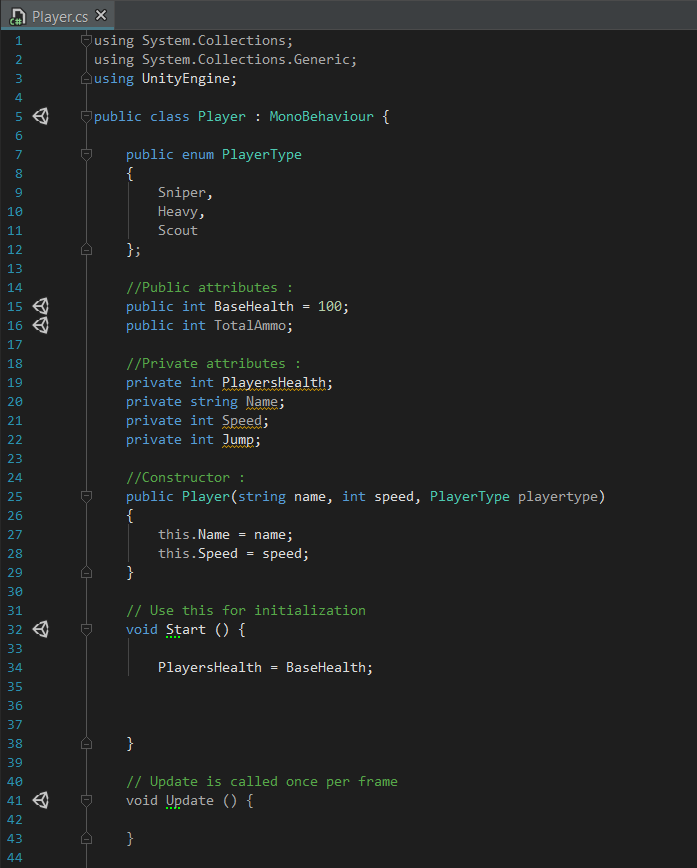
\includegraphics[scale = 0.75]{Script_players.PNG}\\[1cm]
    Script : Players


    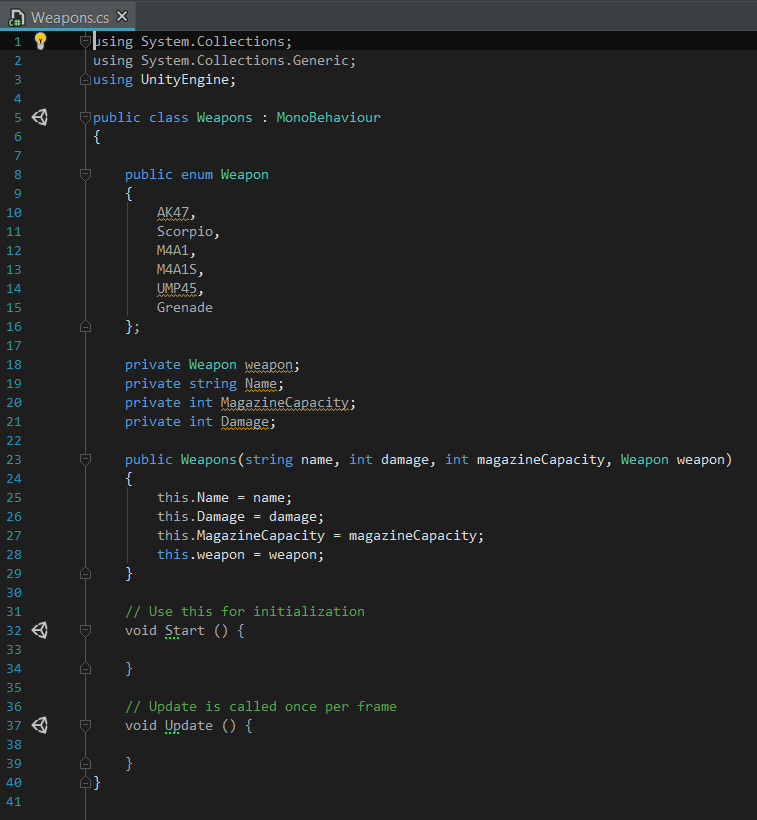
\includegraphics[scale = 0.85]{Script_weapons.PNG}\\[1cm]
    Script : Weapons
    
    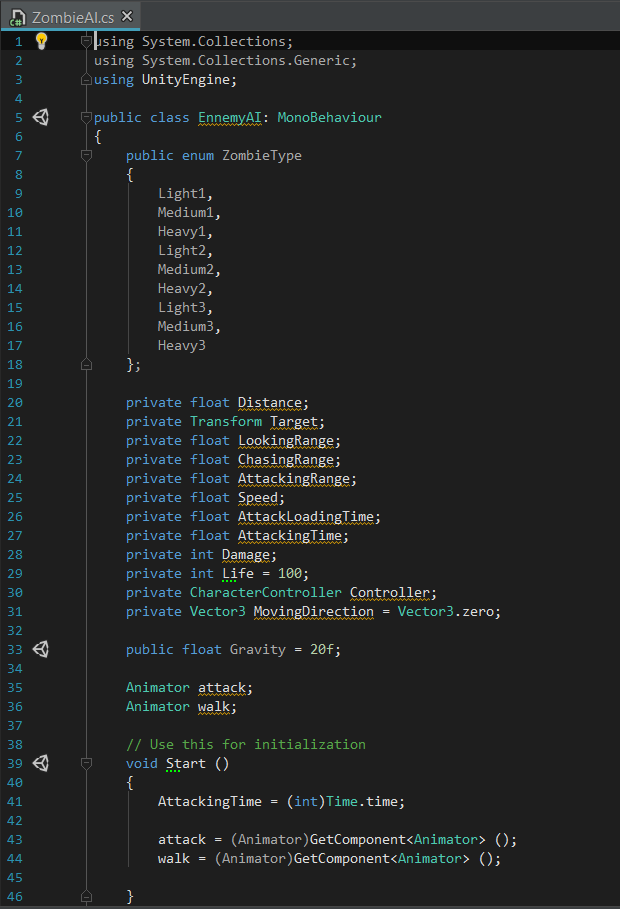
\includegraphics[scale = 0.85]{Script_ZombieAI_-_1.PNG}\\[1cm]
    Script : ZombieAI - part 1
    
    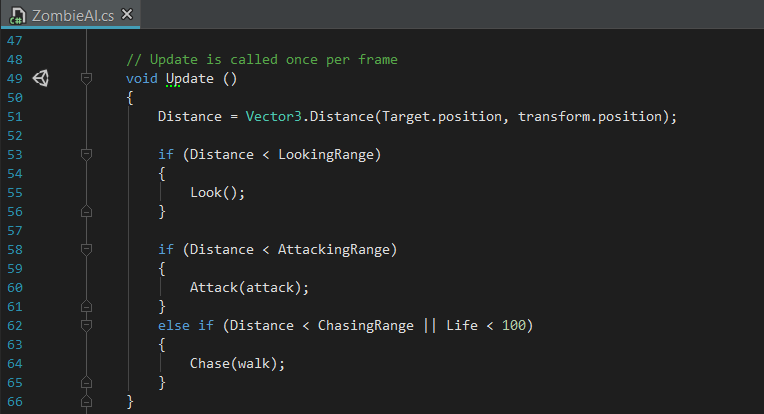
\includegraphics[scale = 0.75]{Script_ZombieAI_-_2.PNG}\\[1cm]
    Script : ZombieAI - part 2
    \bigskip
    
    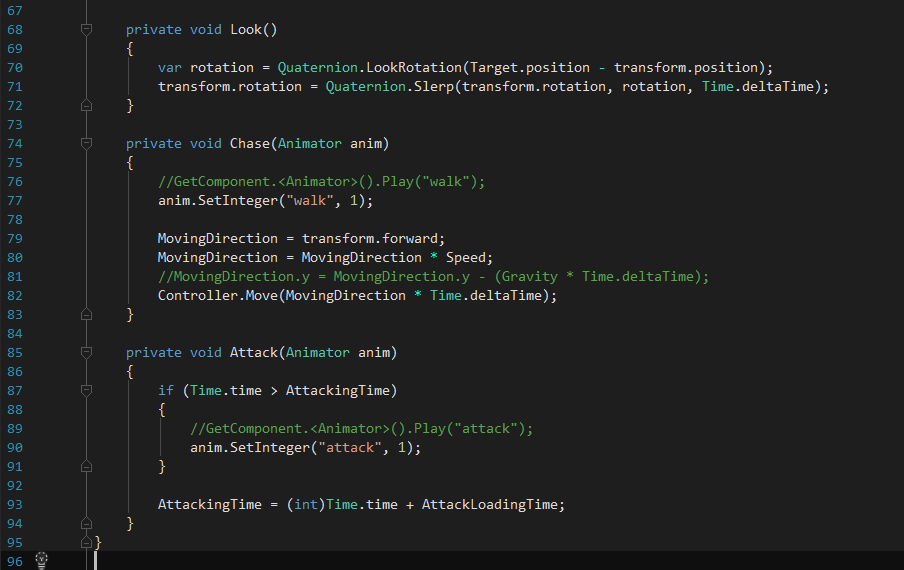
\includegraphics[scale = 0.75]{Script_ZombieAI_-_3.PNG}\\[1cm]
    Script : ZombieAI - part 3
    
    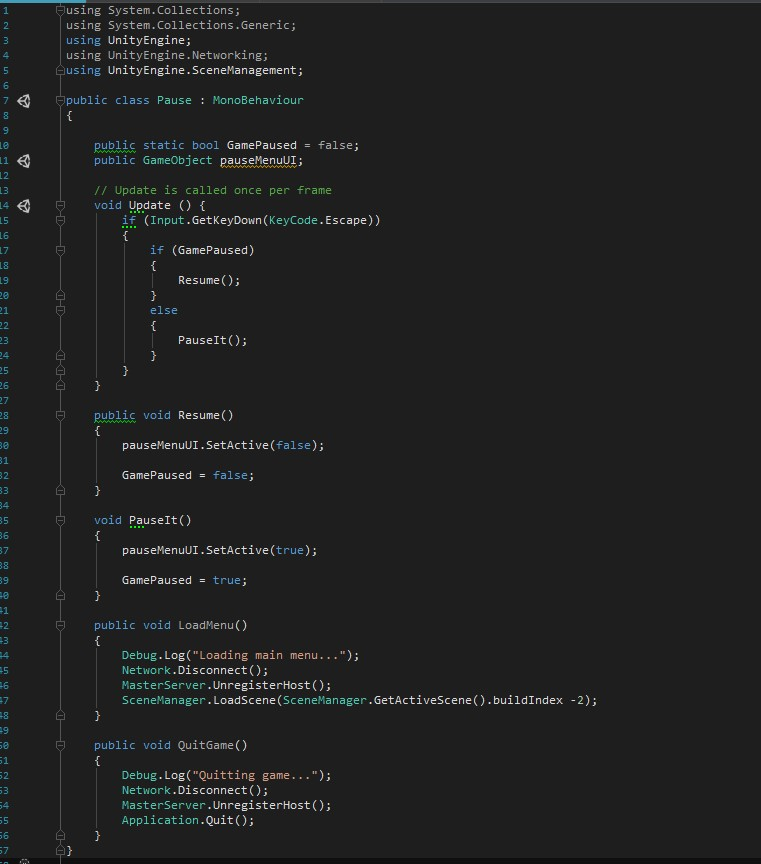
\includegraphics[scale = 0.75]{Pause_script_screen.jpg}\\[1cm]
    Script : Pause menu
   
    % Include a department/university logo - this will require the graphicx package
\end{center}

	\subsubsection{Screenshots}
    
\begin{center}
	\bigskip

	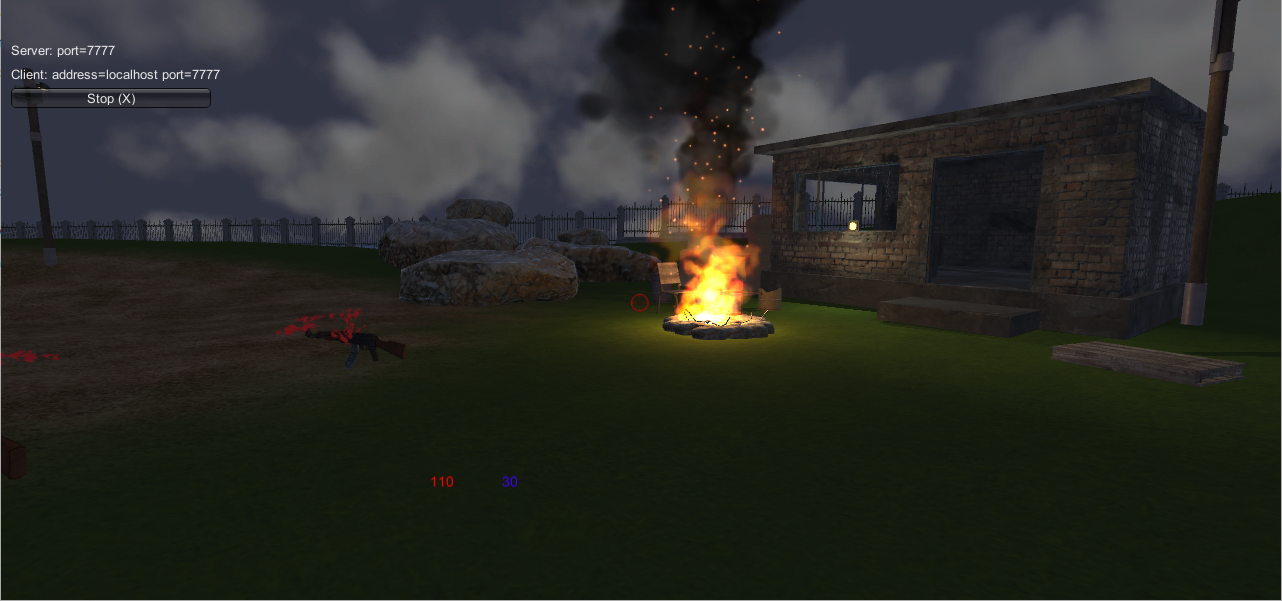
\includegraphics[scale = 0.60]{Campfire.png}\\[1cm]
    Screenshot : Campfire - Spawn point
    
    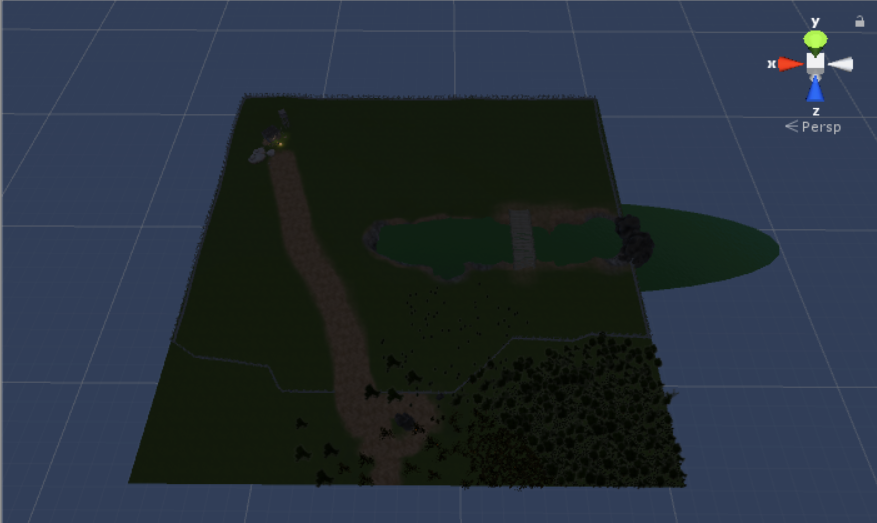
\includegraphics[scale = 0.85]{Map.png}\\[1cm]
    Screenshot : Map - Aerial point of view

   
\end{center}

%----------------------------------------------------------------------------------------
	
    \bigskip
    \bigskip
    
\subsection{Conclusion}

	Thus despite some problems in our group (losing two member and having a new one), along with some programming problems due to the discovery of Unity, we had a good time making the project for this first presentation.//
Building the map, making the gameplay and the AI were few challenges that we overcame, for this first presentation and we are looking forward to facing new challenges.//
For the next presentation we will improve the AI, the animations, the gameplay as well as the sound design, or the website.


\newpage



\begin{center}


 
%----------------------------------------------------------------------------------------
%	HEADING SECTIONS
%----------------------------------------------------------------------------------------

\textsc{\LARGE Computer Project}\\[1.5cm] % Name of your university/college
\textsc{\Large Undergraduate (1st Year) EPITA}\\[0.5cm] % Major heading such as course name
\textsc{\large Report for the 2\ts{nd} Presentation}\\[0.5cm] % Minor heading such as course title


%----------------------------------------------------------------------------------------
%	TITLE SECTION
%----------------------------------------------------------------------------------------

\HRule \\[0.4cm]
{ \huge \bfseries Skraa Party}\\[0.4cm] % Title of your document
\HRule \\[1.5cm]
 
%----------------------------------------------------------------------------------------
%	AUTHOR SECTION
%----------------------------------------------------------------------------------------

\begin{minipage}{0.4\textwidth}
\begin{flushleft} \large
\emph{Co-workers:}\\
Maxime \textsc{Lizandier} % Your name
Ga\'etan \textsc{Diawara}
\end{flushleft}
\end{minipage}
~
\begin{minipage}{0.4\textwidth}
\begin{flushright} \large
\emph{Project Manager:} \\
Yann \textsc{Nitzpon} % Supervisor's Name
\end{flushright}
\end{minipage}\\[2cm]

\end{center}


\newpage

\section{Report of the 2\ts{nd} Presentation}

\subsection{Introduction}
	This report will detail what has been carried out since the last presentation. It details what has been achieved and by whom, but also what needs to be done for the next presentation.
    
\bigskip
\subsection{Precise advancement}
\bigskip
	\subsubsection{The Menus - Maxime}

		The main menu being the first thing we see when running the game, it is a vital element. This is the reason why we completely changed it. We added a new background that was entirely self-made using a graphic tablet. The buttons were also changed along with the audio that is played in a loop, this audio was specifically chosen for the player to get the atmosphere of the game.
\textit{See Appendices : Main menu}
  
        
\bigskip
    \subsubsection{The different parts of the map - Maxime}
    
    	In order to make the game more lively, and to help the player to begin in the game, we created a solo map in which the player will be able to see the different weapons available in the game, the different behaviors of the zombies (basic standing, walking, running and hitting), but also the car that the player will have to repair when playing.\\
\textit{See Appendices : Armory, Zombie box, Shooting range}\\
        
        We also created a map in which the player will spawn for the multiplayer experience. From this part of the map, the players will be able to enter the real multiplayer map in which they will have to face the zombies.\\
\textit{See Appendices : Multiplayer lobby}
        
	\subsubsection{Artificial Intelligence - Ga\'etan \& Yann}
    	Concerning the AI, little changes were made in the scripts, a new method was used so that the zombies can chase the player across the map without hitting anything but the player.\\
        
        Obviously, when only one player is connected, every spawning zombie will run towards this player. But when several players are connected, the zombies that are spawning will randomly choose the player that they will chase.\\
        
        Moreover, once the zombies get hit by a bullet, they play a little animation, and when the player is in hitting range of the zombie, the zombie hits the player and plays the corresponding animation.\\
        
        Finally, when the zombie has less than 25\% of health left, it also plays another animation.\\
\textit{See Appendices : Zombie enemy choice}
\bigskip
    \subsubsection{HUD - Ga\'etan}
    
    	Because for the previous presentation we only had an ugly health and ammunition indicator which were only differentiable by colors (blue and red), we improved the HUD a lot. We now have nice health and ammunition indicators but also an armor indicator (as well as health and ammunition, the player will be able to find armor on the map). These three indicators come with three symbols so they can easily be differentiated.\\
        
        One other feature is the number of the  wave that is displayed according to the current wave.
\bigskip
    \subsubsection{Singleplayer Mode - Maxime}
    
    	In the main menu, once the player clicks on the \guillemotleft \space Singleplayer \guillemotright \space button, he immediately spawns on the solo map in which he will be able to know a little more about the game, it rules and it mechanics.
        
    \subsubsection{Multiplayer Mode - Yann \& Ga\'etan}
    
    	When the player clicks on the main menu's \guillemotleft \space Multiplayer \guillemotright \space button, he spawns in an intermediary map, this map will serve as a lobby, for now, the player will spawn on the real multiplayer map after spending 10 seconds in the lobby.\\
        
        An interesting feature we added in this mode is the different spawn position. In order for the players not to spawn on the same point (so that there won't be any collision problem at the spawn), we created different spawn points. Each player will have his own spawn point once spawning on the map.\\
        Of course, the same principle is applied to the zombies so that when the zombies spawn together, they do not collide.\\
        
        Now one of the most important feature is the one of \guillemotleft \space waves \guillemotright \space. After some time spent on the map, the first wave will begin and three zombies will spawn and and hunt the player(s). Once every zombie has been killed, the wave is finished and after a certain time the next wave is beginning and a bigger amount of zombies spawns.\\
        \textit{See Appendices : Multiplayer network manager}
\bigskip
\subsection{Description of achievements}

	\subsubsection{Our joys}
		One step further in this concrete experience, we took into account that in order to code some feature we wanted to add to our game, we had to do some research, and so each time we improve our game we just learn something new, and this is what we found very interesting about this project.\\
        What is also nice is the set of tools that Unity already has, like the Unity Networking (UNET) tool that made it really easy to code the multiplayer mode.\\
        Moreover, as we could use other softwares than Unity, we could overcome the parts we didn't like doing in unity.For the map building for example, we used ProBuilder and for the menu creation we used Krita.\\
\newpage
		Finally, one big advantage is that we could find a lot of assets on the Internet, that is to say every asset we used, from the map creation to the muzzle flash without forgetting the different characters and their animations.\\
        
        Some of us preferred the coding part (which they really enjoy) and others are more into the graphic and map building part. But at the end we all enjoyed the work we did.
        
%\newpage
\bigskip
	\subsubsection{Our sadness}
		One counterpart of downloading assets from the Internet is that they sometimes have little texture problems or have a bad time adapting to our project (in particular the animations).\\
        
        But really, the main sadness for us was every problem we encountered because of the project sharing, we first used \guillemotleft \space Unity collab \guillemotright \space, but it only allows for 1GB of data, so we then used \guillemotleft \space GitHub \guillemotright \space, but every import had to be less than 100MB, which after sometime was not a problem anymore. However we still had a lot of problems due to GitHub Desktop and compiling errors.
\bigskip
\subsection{What still needs to be done}
    
    \subsubsection{Progression}
\bigskip
\scalebox{0.85}{
\begin{tabular}{|l|c|c|c|} 
	\hline
    \textbf{Tasks} & \textbf{1\ts{st} Presentation} & \textbf{2\ts{nd} Presentation} & \textbf{Final Presentation} \\
    \hline
    Menus creation & 30 \% & 75 \%  & 100 \% \\
    \hline
    Map design & 30 \% & 60 \% & 100 \% \\
    \hline
    3D element creation & 10 \% & 40 \% & 100 \% \\
    \hline
    HUD & 20 \% & 50 \% & 100 \% \\
    \hline
    Game scenario \& story & 30 \% & 75 \% & 100 \% \\
    \hline
    Gameplay \& pathing & 30 \% & 75 \% & 100 \% \\
    \hline
    Visual effects & 20 \% & 50 \% & 100 \% \\
    \hline
    Sound design & 30 \& & 75 \% & 100 \% \\
    \hline
    Website & 30 \% & 60 \% & 100 \% \\
    \hline
    Online mode & 20 \% & 50 \% & 100 \% \\
    \hline
    Service Provider (Network, domain name) & 75 \% & 100 \% & 100 \% \\
    \hline
    AI & 20 \% & 50 \%  & 100 \% \\
    \hline
    
\end{tabular}}
\bigskip

    \subsubsection{Map building}
    
    	In the solo map, we still need to add the different characters that the player could possibly choose in the multiplayer mode, they would be shown between the zombie and the weapons.\\
        In the \guillemotleft \space multiplayer lobby \guillemotright \space as we call it, we want to add a \guillemotleft \space Non-player character \guillemotright \space (NPC) in order for the player to interact with it (more information about that a bit further).
        Now in the multiplayer map, we might add some elements or building, but we will mainly add the health, armor and ammunition elements along with the different car parts the player will need to escape.
\bigskip
    \subsubsection{Menu settings}
    
    	In the main menu, we could add some other features in the settings window, like the key binds for the azerty or qwerty keyboards.
\bigskip 
    \subsubsection{Gameplay}
    	
        As stated before, we want to add a NPC in the multiplayer lobby so that the players could interact with it, this is to say they will be able to choose the character they want to play with. And after we will have added the \guillemotleft \space money earning \guillemotright \space system (after each game, the player will earn some amount of money depending of the number of kills he made), the player will be able to use the shop feature of the NPC, with which he will be able to improve his weapons.\\
        In this lobby, the player will also be able to choose the game they want to enter, so that if ten players are in the main lobby, three friends will be able to play together in the same lobby without the other players.
\bigskip   
    \subsubsection{HUD}
        
    	For the HUD part, we might also make some changes, they will mainly be for aesthetic purposes, but we will add the number of kills the player made during the current game. 
        
\subsection{Appendices}

    \subsubsection{Screenshots}
    
    \bigskip
\begin{center}	
	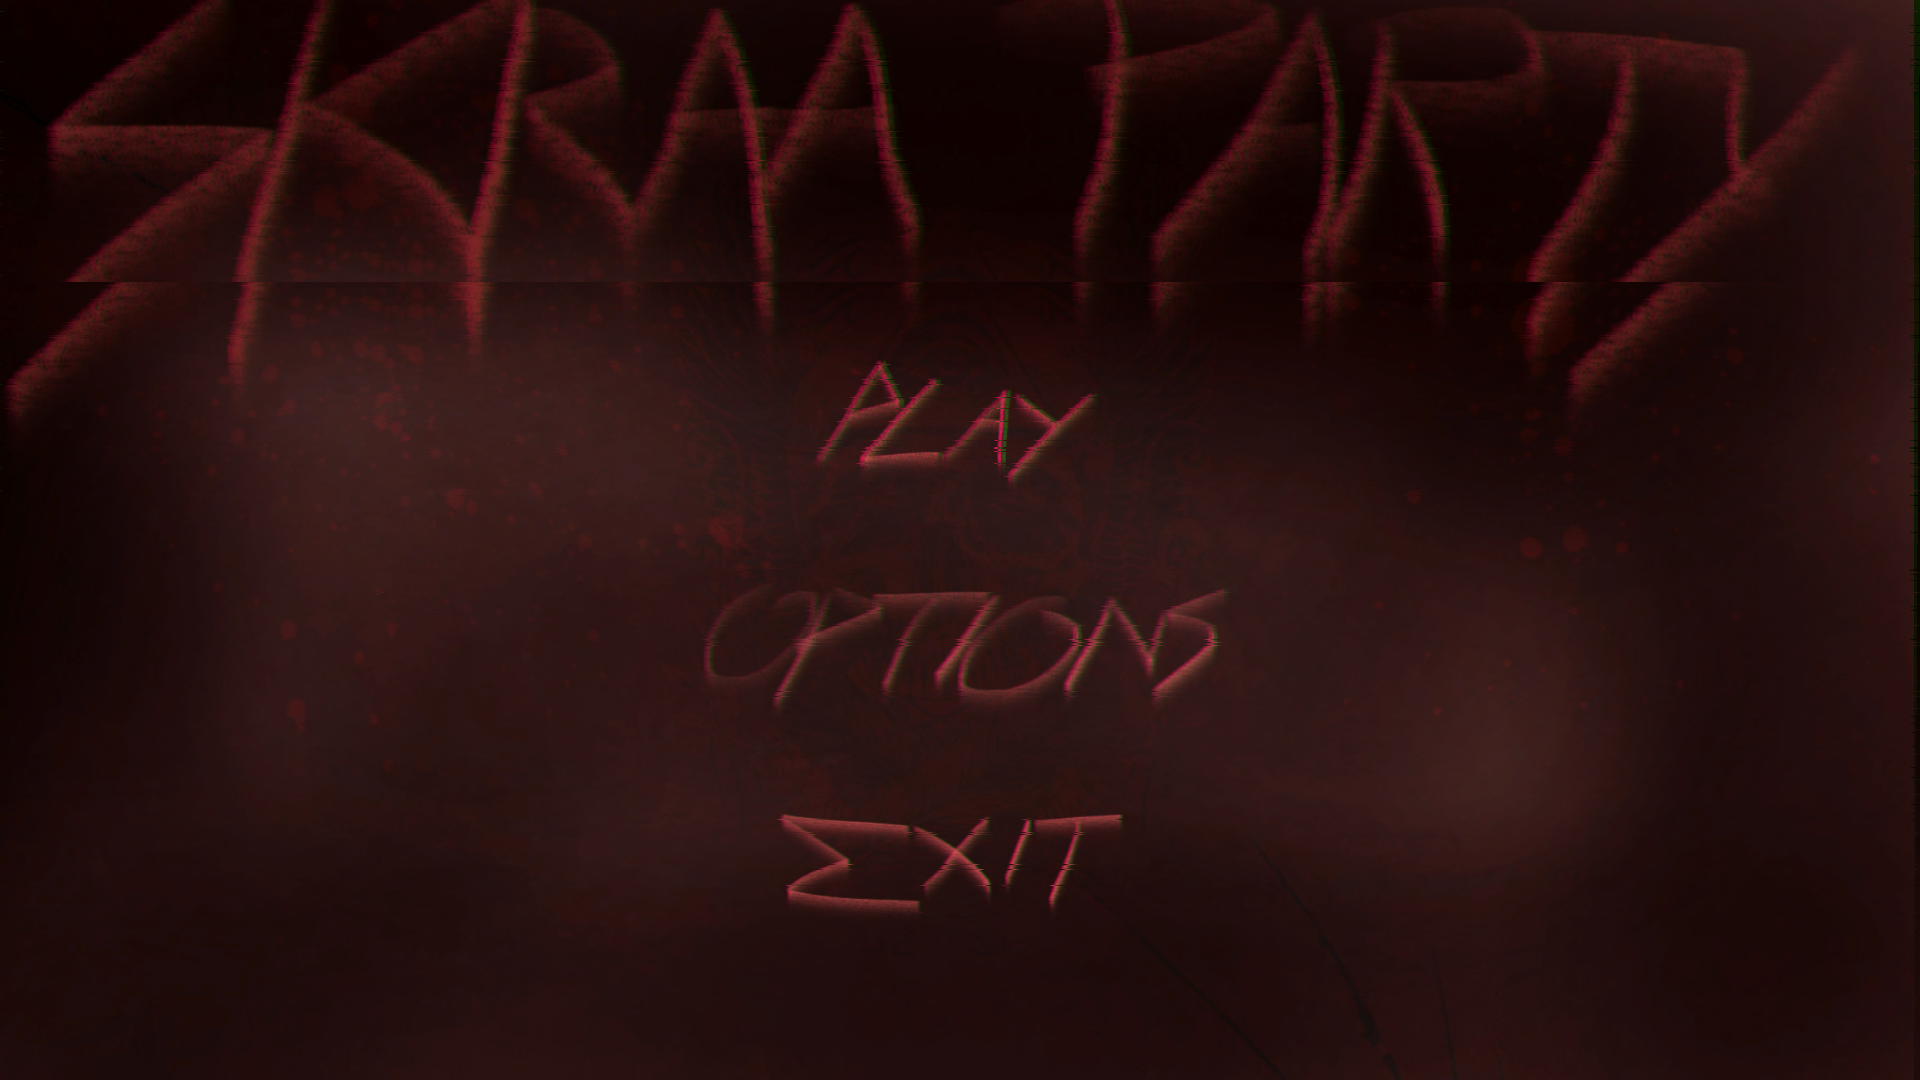
\includegraphics[scale = 0.40]{Main_menu.PNG}\\[1cm]
    Screenshot : Main menu
\end{center}
\newpage
\begin{center}	
	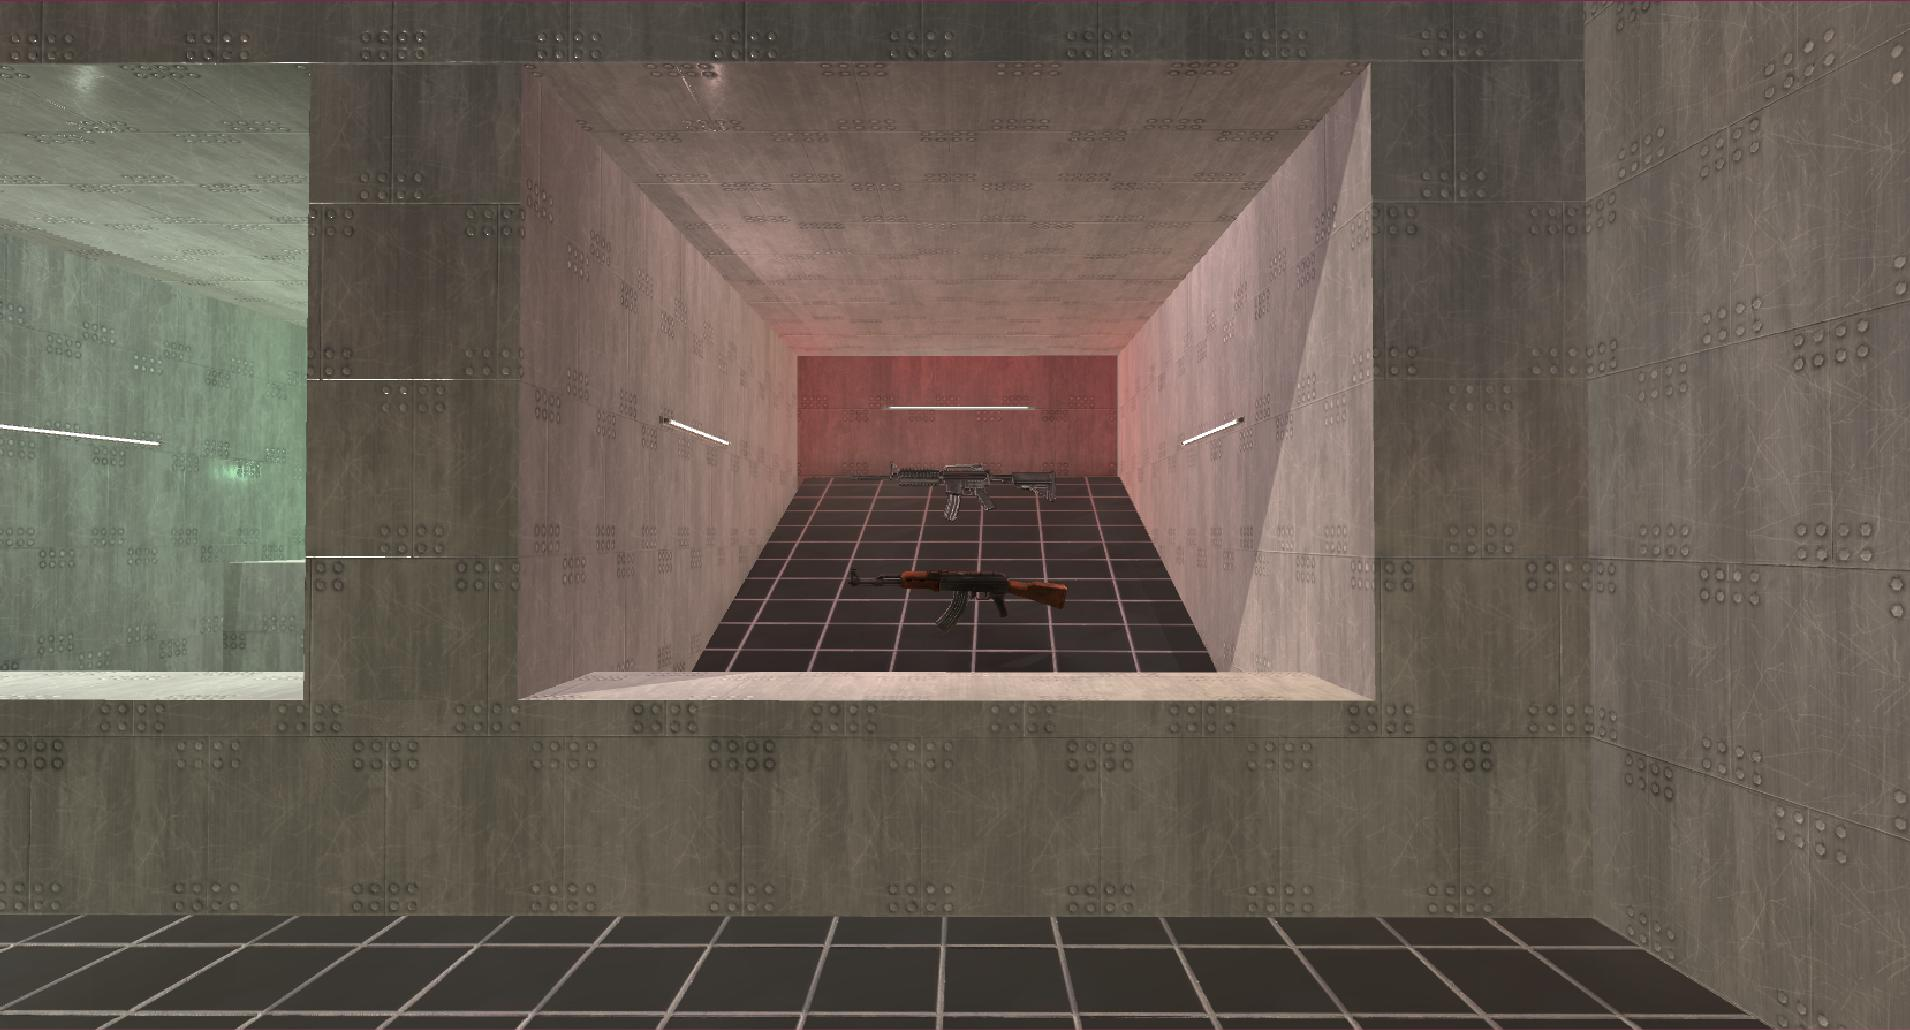
\includegraphics[scale = 0.60]{Screen_Armes-ConvertImage.jpg}\\[1cm]
    Screenshot : Armory
\end{center}
\newpage
\begin{center}	
	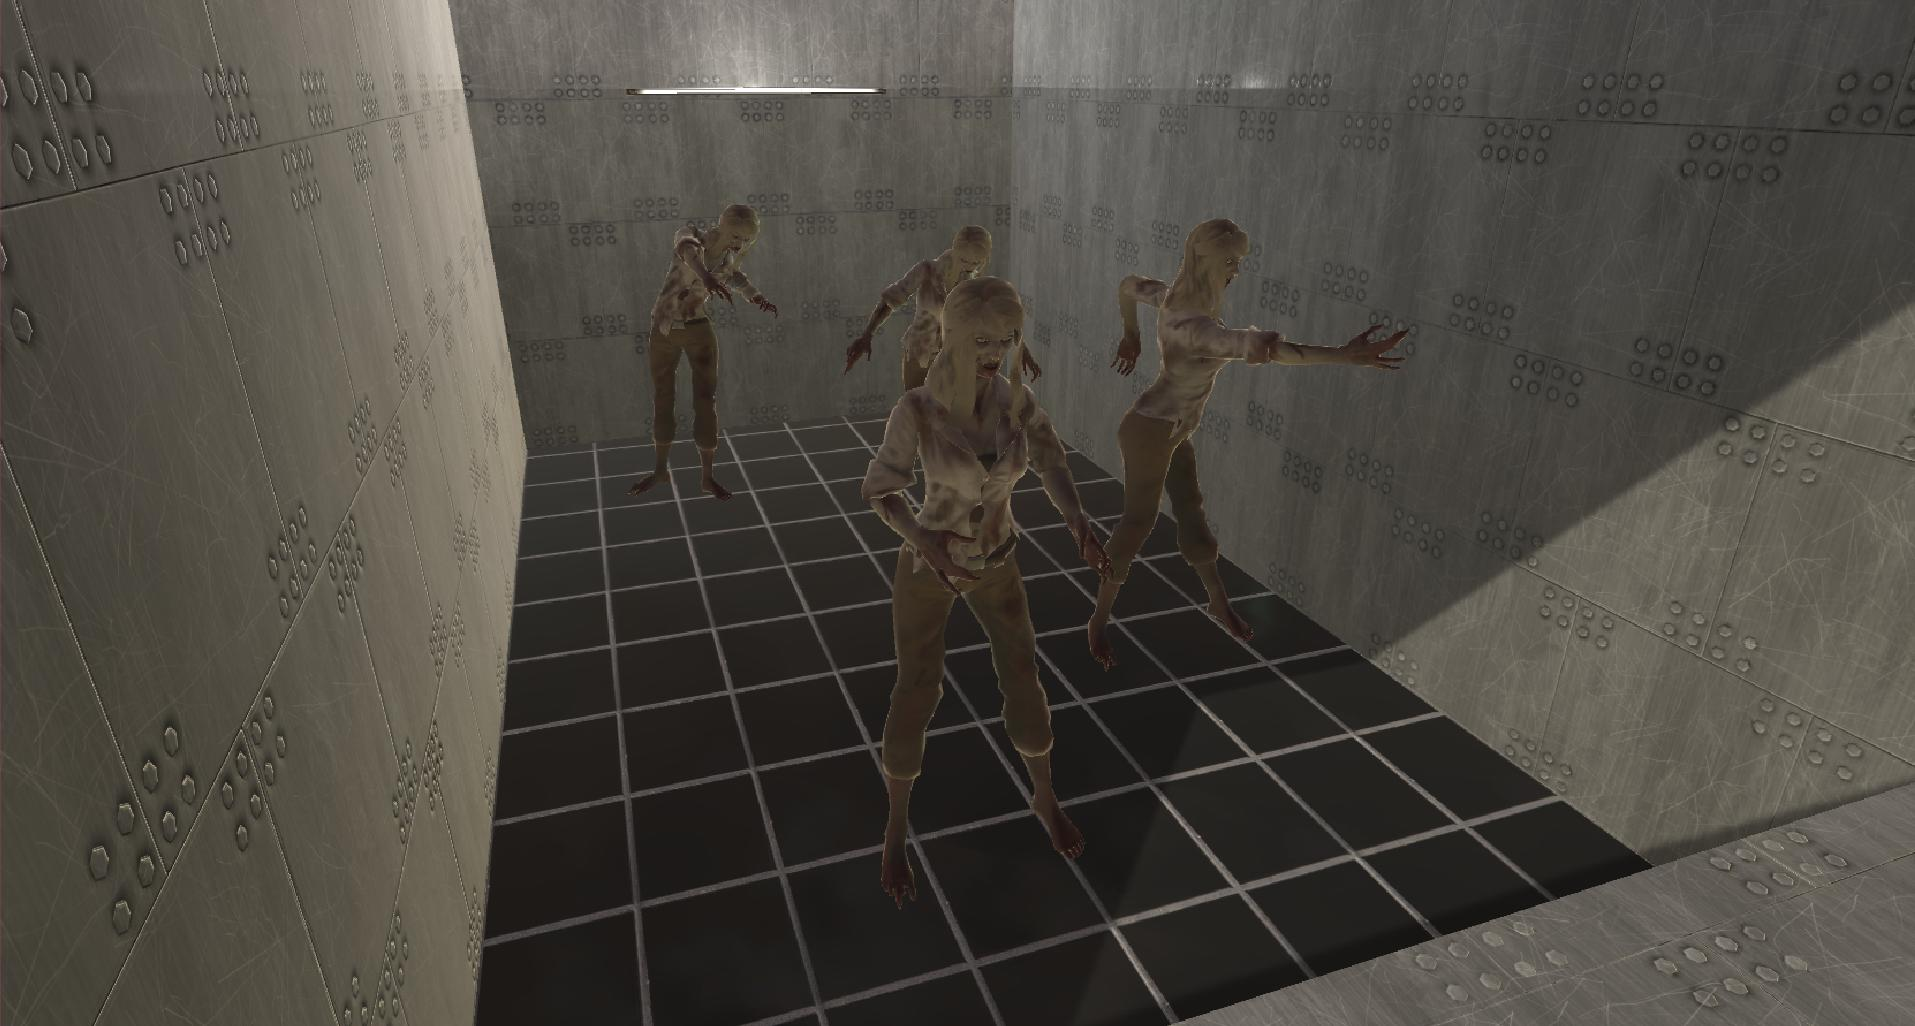
\includegraphics[scale = 0.60]{Screen_Zombies-ConvertImage.jpg}\\[1cm]
    Screenshot : Zombie box
\end{center}
\newpage
\begin{center}	
	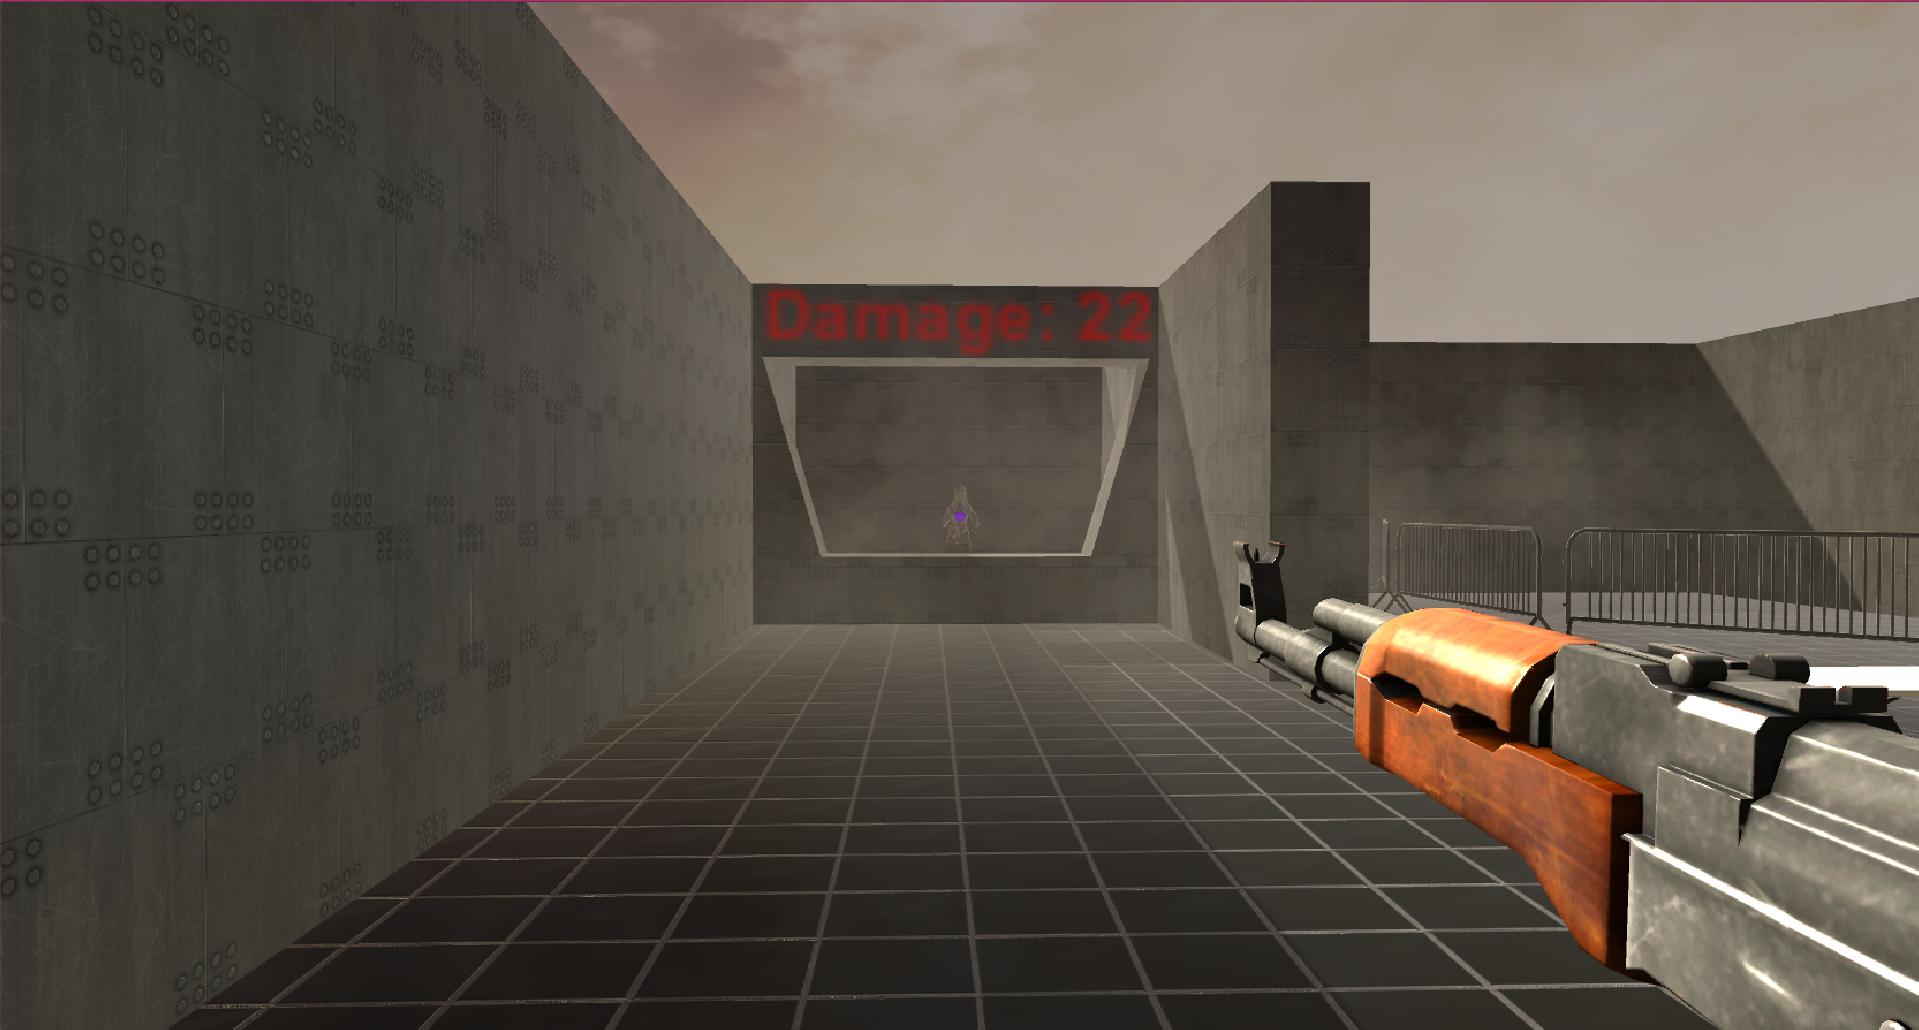
\includegraphics[scale = 0.60]{Screen_Damage-ConvertImage.jpg}\\[1cm]
    Screenshot : Shooting range
\end{center}
\newpage
\begin{center}	
	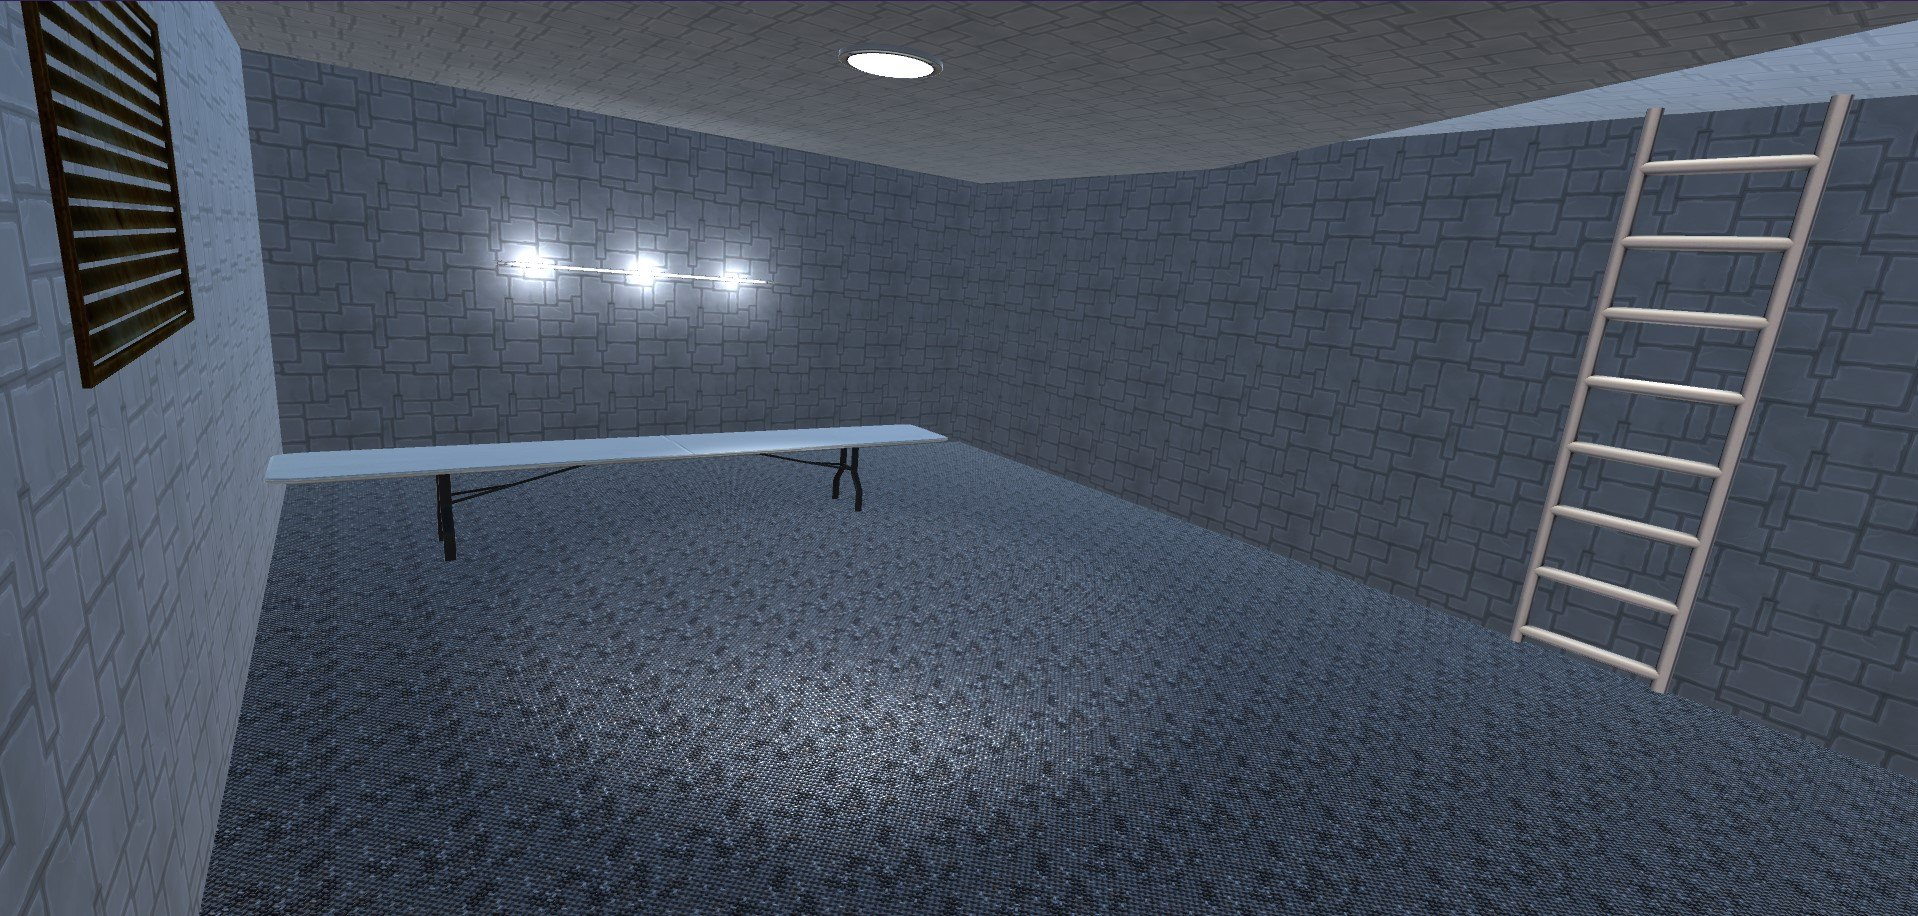
\includegraphics[scale = 0.25]{Multiplayer_lobby.jpg}\\[1cm]
    Screenshot : Multiplayer lobby
\end{center}
\newpage
\begin{center}	
	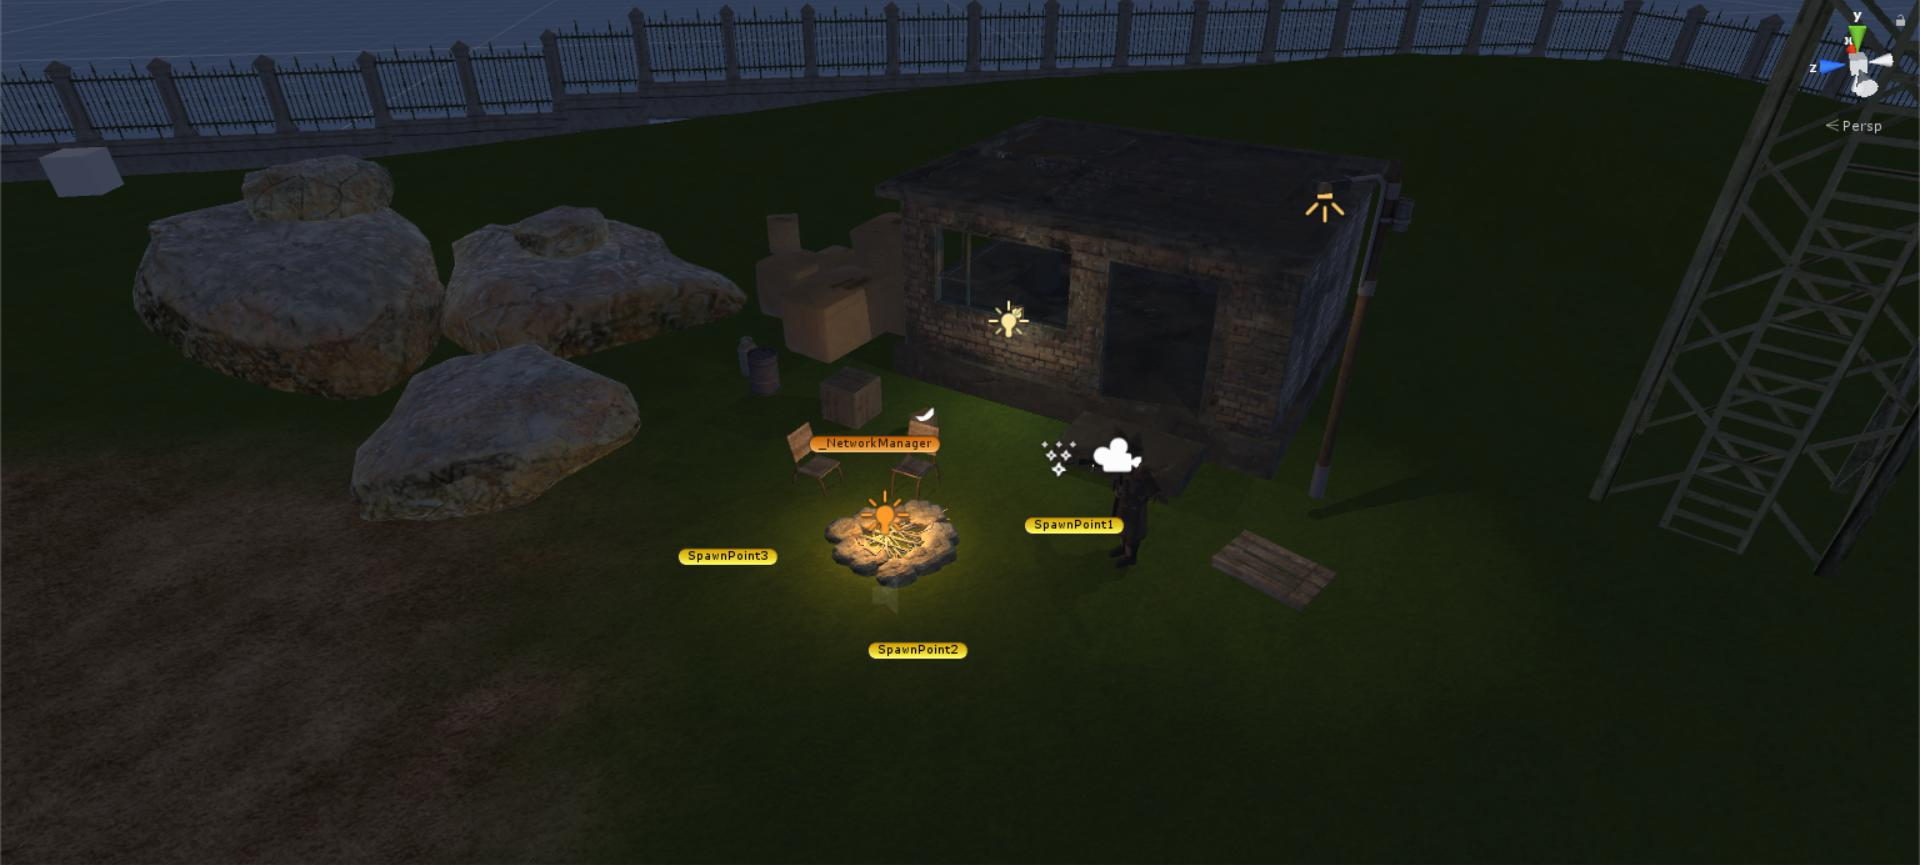
\includegraphics[scale = 0.60]{Network-Manager-ConvertImage.jpg}\\[1cm]
    Screenshot : Multiplayer network system
\end{center}
\newpage

	\subsubsection{Scripts}
    
\begin{center}	
	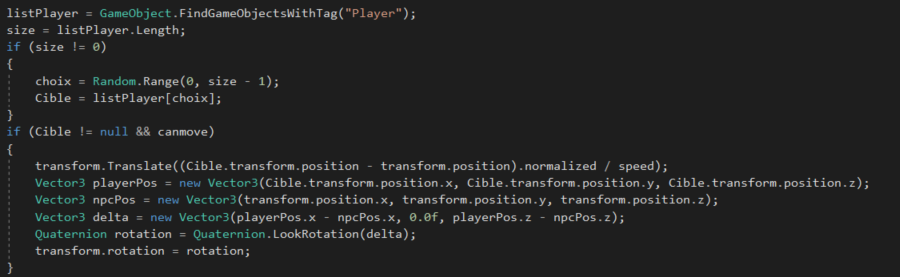
\includegraphics[scale = 0.50]{looking_func.png}\\[1cm]
    Screenshot : Looking function of the zombies
\end{center}

\begin{center}	
	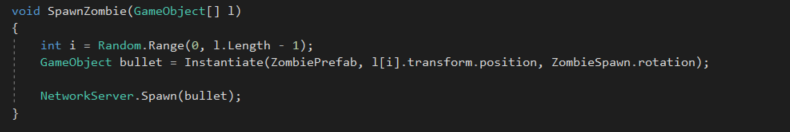
\includegraphics[scale = 0.60]{Zombi_spawn.png}\\[1cm]
    Screenshot : Zombie spawning function
\end{center}
\newpage

\subsection{Conclusion}
	During this period of time (since the first presentation) we learned a tremendous amount of things about video game programming.
    Despite this learning, we still struggled a lot, especially with the sharing of the project (with GitHub Desktop).
    However we still succeeded in improving our game, whether concerning the menus, the HUD, the AI, or even the gameplay of the whole game.
    
\newpage



\begin{center}


 
%----------------------------------------------------------------------------------------
%	HEADING SECTIONS
%----------------------------------------------------------------------------------------

\textsc{\LARGE Computer Project}\\[1.5cm] % Name of your university/college
\textsc{\Large Undergraduate (1st Year) EPITA}\\[0.5cm] % Major heading such as course name
\textsc{\large Report for the 3\ts{rd} Presentation}\\[0.5cm] % Minor heading such as course title


%----------------------------------------------------------------------------------------
%	TITLE SECTION
%----------------------------------------------------------------------------------------

\HRule \\[0.4cm]
{ \huge \bfseries Skraa Party}\\[0.4cm] % Title of your document
\HRule \\[1.5cm]
 
%----------------------------------------------------------------------------------------
%	AUTHOR SECTION
%----------------------------------------------------------------------------------------

\begin{minipage}{0.4\textwidth}
\begin{flushleft} \large
\emph{Co-workers:}\\
Maxime \textsc{Lizandier} % Your name
Ga\'etan \textsc{Diawara}
\end{flushleft}
\end{minipage}
~
\begin{minipage}{0.4\textwidth}
\begin{flushright} \large
\emph{Project Manager:} \\
Yann \textsc{Nitzpon} % Supervisor's Name
\end{flushright}
\end{minipage}\\[2cm]

\end{center}

\newpage

\section{Report of the 3\ts{rd} (Final) Presentation}

	\subsection{Introduction}

	This final report will remind what we planned for our game to be like, everything we wanted it to contain, and then it will detail our latest advancement and some things we added on the run.
    
    \subsection{Our initial goal}

	Since the beginning, what we wanted to create was fun game to play, with a \guillemotleft \space coherent \guillemotright \space scenario. The game would mostly consist of the multiplayer experience but the player should also be able to play alone.\\
    When the player spawns on the map (alone or with other players) he can first take a look at the map. There are different buildings and elements (such as the lake, the bridge, trees, street lights, and many other) that add to the atmosphere we wanted our game to have. But there should also be some perks the player can pick-up, these are ammunition, health and armor. One key point we wanted our game to have was the car the player would have to  repair in order to escape the zombie filled park. We thought the game should be interesting and intuitive, hence the HUD, the player should always know how much life, armor and ammunition he has. The other key point we wanted was the system of waves, the zombies should spawn on the map following a certain pattern, preventing the player to have too many zombies against him at once but enough to seriously challenge his skills.
    
    \subsection{Precise advancement}
    	
        \subsubsection{The Menus - Maxime}
        
        We decided to keep the design of the main menu (which we still love), but we add another button, the \guillemotleft \space About the game \guillemotright \space button, which allows the player to see the trailer of the game but also the credits section.\\
        The other menus such as the in-game menus should stay as they were, at least for the elements. But we added a higher opacity to the background to decrease the contrast between the menu and the game.\\
        %\textit{See Appendices : Final Main menu, Final in-game menu}\\
        
        \subsubsection{The different parts of the map - Maxime, Yann and Ga\'etan}
        
        First for the solo map, the improvements we made are those we planned to do, that is to say the adding of the car model the player will have to repair, and the repair pieces, which are all shown in the corner of the map, behind the barriers. But also the different characters the player will be able to choose when playing in the multiplayer mode, the player is able to see them between the zombie and the weapons.\\
        Now for the multiplayer lobby, as we planned, we added a \guillemotleft \space Non-player character \guillemotright \space (NPC). The player is able to interact with it, he can choose the game lobby he wants to play in with the other player of his choice. The player can also upgrade some of his weapons in order for them do make more damage, and he can choose the character we wants to embody for the multiplayer experience.\\
        At last for the multiplayer map, we added the car the player has to repair in order to escape and of course the car pieces he needs to repair it, therefore he will be able to pick them them up on different places of the map.\\
        \textit{See Appendices : Solo Map Escape car/truck, Multiplayer map (1, 2, 3)}
        
        \subsubsection{Menu settings - Maxime}
        
        As we said we would, we added the two different keyboards layouts so that the player can choose to play with the AZERTY layout or the QWERTY one.
        
        \subsubsection{Gameplay - Yann}
        
        As written before, the player is now able to interact with the NPC in order to choose the character he wants to play with and to upgrade his weapons, all this thanks to the in-game money. The player wins this money after each game he played, depending on the number of kills he made during each game.\\
        
        \subsubsection{HUD - Ga\'etan}
        
        We added the kill counter (which obviously shows the number of kills made during the current game).\\
        
	\subsection{Description of achievements}
        
        \subsubsection{Our joys}
        
        Once more, we liked coding an actual concrete project in which one rule stands : \guillemotleft \space You want some new feature in your game, you implement it \guillemotright, that is to say that the ideas we had, as long as there were realistic, we followed them and add them to the game. Despite the fact that Maxime and Yann had never used Unity at all at the beginning of the project, they were able to create and give life to their ideas (as did Ga\'etan), of course it requires a lot of research, but it actually is possible to \guillemotleft \space do what you want \guillemotright.
        
        \subsubsection{Our sadness}
        
        \textit{This project has reached an end, and this is sad, isn't it enough already !!}\\
        
        More seriously, we still had a hard time with the file sharing and merging, we found the trick at the end, but until that moment we really took it upon ourselves not to smash something up.
        
    \subsection{To summarize}
    
    So, at the end we have a well working game. When the player starts the game, he sees a beautiful menu from which he can choose either to play the singleplayer mode, to dare the multiplayer experience, to see more about the game or\... to exit the game (but let's focus on the three first choices).\\
    When clicking the Singleplayer button, the player is redirected to the solo map, he can see the different weapons and characters available for the multiplayer mode, the different behaviors of the zombies he will have to face, the car he will have to repair in order to escape the park, and train his aim at the shooting range.\\
    Now when selecting the multiplayer button, the player is sent to the multiplayer lobby, from there he can : interact with the NPC and choose in which lobby he wants to wait/play, upgrade his weapons, and choose the character he wants to embody for the game. When the game is launched, the player spawns on the map near the fire-camp. The map is composed of natural elements (a lake, trees, and rocks), some buildings, and other elements such as street lights, item to pick-up like weapons, health, armor, ammunition and car pieces, and the car that goes with it (some elements are more useful than others - we agree). At one point, the first wave of zombies appears, as the player will notice thanks to the wonderful HUD we have, that shows the current health, armor and ammunition available along with the current wave number and the kill counter. The player hast to kill every zombie on the map in order to finish the wave, and as long as the wave is not finished, he can't repair the car, even if he found some parts. The more waves the player reaches, the more zombies arrive (else it wouldn't be realistic). Once the car is fully repaired, the player can escape and he wins the game, along with a whole bunch of money.
        
    \subsection{Possible further upgrade}
    
    Of course we also had some other ideas, but not all the time we wanted/needed to make them appear in the game. The player could be able to purchase other characters (to embody in the multiplayer experience) with in-game money.
    
    \subsection{Appendices}
    
    	\subsubsection{Screenshots}
        
            \newpage
            \begin{center}	
            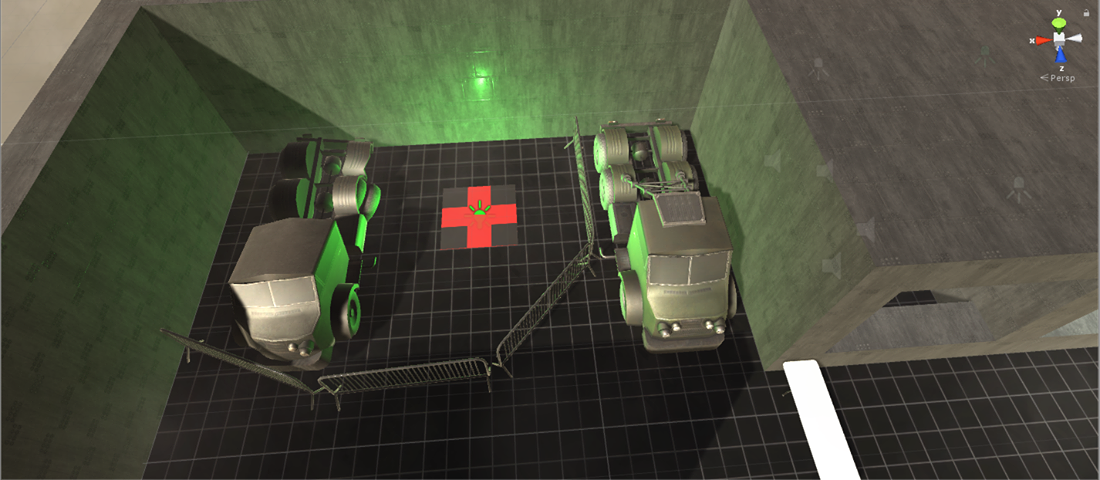
\includegraphics[scale = 0.40]{Solo_Map_Truck.png}\\[1cm]
            Screenshot : Solo map escape car/truck
            \end{center}
            \newpage
            
            \begin{center}	
            \includegraphics[scale = 0.65]{dzqdqzsxwww.PNG}\\[1cm]
            Screenshot : Multiplayer map (1)
            \end{center}
            \newpage
            
            \begin{center}	
            \includegraphics[scale = 0.65]{yannf.PNG}\\[1cm]
            Screenshot : Multiplayer map (2)
            \end{center}
            \newpage
            
            \begin{center}	
            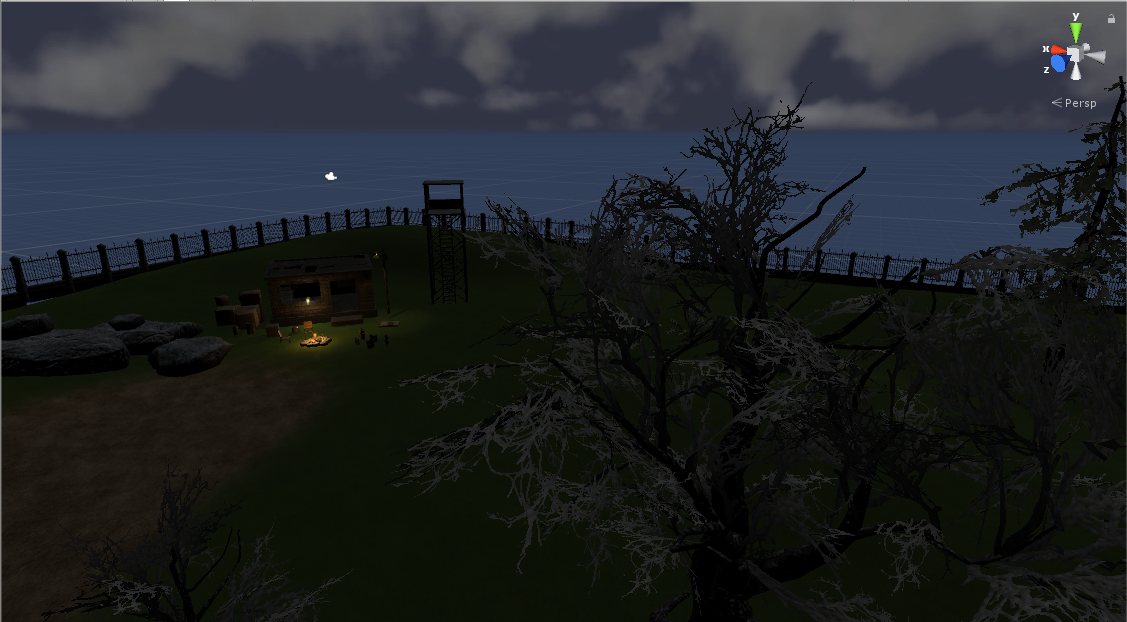
\includegraphics[scale = 0.65]{zeaqeza.PNG}\\[1cm]
            Screenshot : Multiplayer map (3)
            \end{center}
            \newpage
        
        %\subsubsection{Scripts}
        
        
    \subsection{Bibliography and Webography}
    
    	\subsubsection{Websites}
        
        	Unity User Manual : \url{https://docs.unity3d.com/Manual/UnityManual}\\
            Open Classroom : \url{https://openclassrooms.com/courses/realisez...}
            GitHub - KinoGlitch : \url{https://github.com/keijiro/KinoGlitch}
            
        \subsubsection{Forums}
        
        	Forum Unity3D-France : \url{http://www.unity3d-france.com/unity/phpBB3/index.php}
            
        \subsubsection{Video Tutorials}
        
        	Overall Unity tutorials : \url{https://www.youtube.com/user/brackeys}\\
            TUTO UNITY FR : \url{https://www.youtube.com/channel/UCJRwb5W4Z...}\\
        	Unity Navigation Mesh : \url{https://www.youtube.com/user/ryandome}\\

\end{document}
